\documentclass[tikz,border=4pt]{standalone}
\usetikzlibrary{arrows.meta,positioning}
\definecolor{edaink}{HTML}{13263D}
\definecolor{edablue}{HTML}{2563A6}
\definecolor{edateal}{HTML}{16736A}
\definecolor{edaviolet}{HTML}{7756A5}
\definecolor{edaamber}{HTML}{B45309}
\tikzset{
  edabox/.style={draw, rounded corners=2pt, line width=.7pt,
    minimum height=9mm, text width=24mm, align=center, inner sep=2pt,
    text=edaink, font=\sffamily\small},
  front/.style={edabox, draw=edablue, fill=edablue!8},
  verify/.style={edabox, draw=edaviolet, fill=edaviolet!8},
  physical/.style={edabox, draw=edateal, fill=edateal!8},
  release/.style={edabox, draw=edaamber, fill=edaamber!8},
  edaflow/.style={-{Latex[length=2mm]}, line width=.7pt, draw=edaink},
  edafeedback/.style={edaflow, dashed, draw=edaamber},
  edalabel/.style={font=\sffamily\scriptsize, text=edaink}
}

\begin{document}
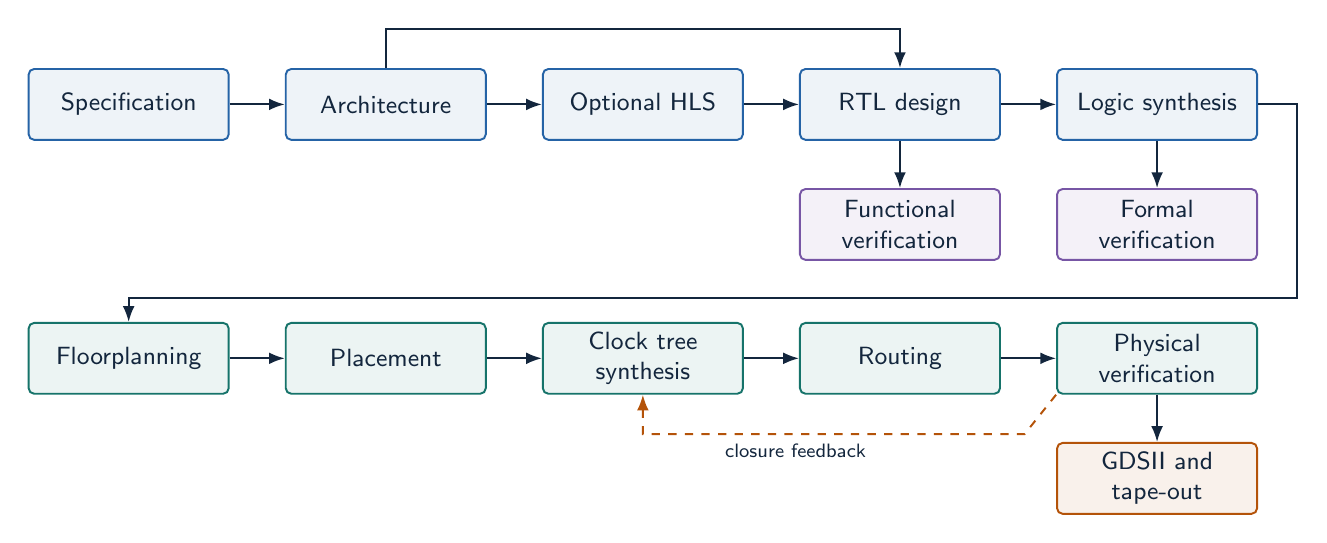
\begin{tikzpicture}[node distance=6mm and 7mm]
  \node[front] (spec) {Specification};
  \node[front, right=of spec] (arch) {Architecture};
  \node[front, right=of arch] (hls) {Optional HLS};
  \node[front, right=of hls] (rtl) {RTL design};
  \node[front, right=of rtl] (synth) {Logic synthesis};
  \node[verify, below=of rtl] (sim) {Functional verification};
  \node[verify, below=of synth] (formal) {Formal\\verification};
  \node[physical, below=23mm of spec] (floor) {Floorplanning};
  \node[physical, right=of floor] (place) {Placement};
  \node[physical, right=of place] (cts) {Clock tree synthesis};
  \node[physical, right=of cts] (route) {Routing};
  \node[physical, right=of route] (signoff) {Physical verification};
  \node[release, below=of signoff] (gds) {GDSII and tape-out};

  \foreach \from/\to in {spec/arch,arch/hls,hls/rtl,rtl/synth,rtl/sim,
    synth/formal,floor/place,place/cts,cts/route,route/signoff,signoff/gds}
    \draw[edaflow] (\from) -- (\to);
  \draw[edaflow] (arch.north) -- ++(0,5mm) -| (rtl.north);
  \draw[edaflow] (synth.east) -- ++(5mm,0) |- ([yshift=3mm]floor.north) -- (floor.north);
  \draw[edafeedback] (signoff.south west) -- ++(-4mm,-5mm)
    -| node[pos=.3,below,edalabel] {closure feedback} (cts.south);
\end{tikzpicture}
\end{document}
